\documentclass{beamer}
\usetheme{metropolis}
\title{The Cipher Challenge}
\subtitle{Cryptanalysis for classical cryptography}
\author{Izaak van Dongen}
\institute{Hills Road SFC}
\date{\today}

\AtBeginSection{\frame{\sectionpage}}
\AtBeginSubsection{\frame{\subsectionpage}}
\AtBeginSubsubsection{\frame{\subsubsectionpage}}

\usepackage{booktabs}

% listings of code
\usepackage{minted}
\setminted{breaklines,
           breakbytokenanywhere,
           linenos
}
\usemintedstyle{friendly}
% bigger line numbers
\renewcommand\theFancyVerbLine{\footnotesize\arabic{FancyVerbLine}}

% that can break across pages while being captioned figures
\usepackage{caption}
\newenvironment{longlisting}
{\addvspace{\baselineskip}\captionsetup{type=listing}}
{\addvspace{\baselineskip}}

\usepackage{mathtools}

\begin{document}
\begin{frame}
    \titlepage
\end{frame}

\begin{frame}
    \frametitle{Outline}
    \tableofcontents
\end{frame}

\section{Statistics}

\begin{frame}
\frametitle{Strategy}

We take the English letter distribution \footnote{
    http://en.algoritmy.net/article/40379/Letter-frequency-English
} to be roughly invariant:

\begin{tabular}{l|ccccccccccc}
$L$ & E & T & A & O & I & N & S & H & R & D & \ldots \\
$P(L)/\%$ & 13 & 9.1 & 8.2 & 7.5 & 7 & 6.7 & 6.3 & 6.1 & 6 & 4.3 & \ldots\\
\end{tabular}

\end{frame}

\begin{frame}[fragile]
\frametitle{Index Of Coincidence}

This implies that the IOC will also be invariant. IOC can be calculated as:

$\text{IOC} = \sum\limits_{r=0}^{25} \frac{n_r(n_r - 1)}{N(N - 1)}$
\begin{minted}[fontsize=\footnotesize]{python}
def ioc(count: collections.Counter):
    total = sum(count.values())
    return (sum(freq ** 2 - freq for freq in count.values())
         / (total ** 2 - total))
\end{minted}

In English, this is expected to be around 0.06654.

\end{frame}

\begin{frame}
\frametitle{Fitness metrics}

We can measure the closeness of some text to English (its ``fitness'') in
several ways.

One is to take its letter distribution as a vector in 26 dimensions. It is
normalised such that the sum of its components is equal to 1. We can then take
the total deviance of this distribution from the expected English distribution
as a measure of fitness.

Another approach is by quadgrams. We take every four adjacent letters and look
up the expected frequency of this combination in a large table of every $26^4$
quadgrams. We use this to judge how similar we think the text is to English.
\end{frame}

\section{Monoalphabetic substitution ciphers}

\subsection{The Caesar cipher}

\begin{frame}
\frametitle{The Caesar cipher}
The Caesar cipher is normally thought of as a simple shift, or rotation, of each
letter.

\begin{center}
\begin{minipage}{6in}
  \raisebox{-0.5\height}{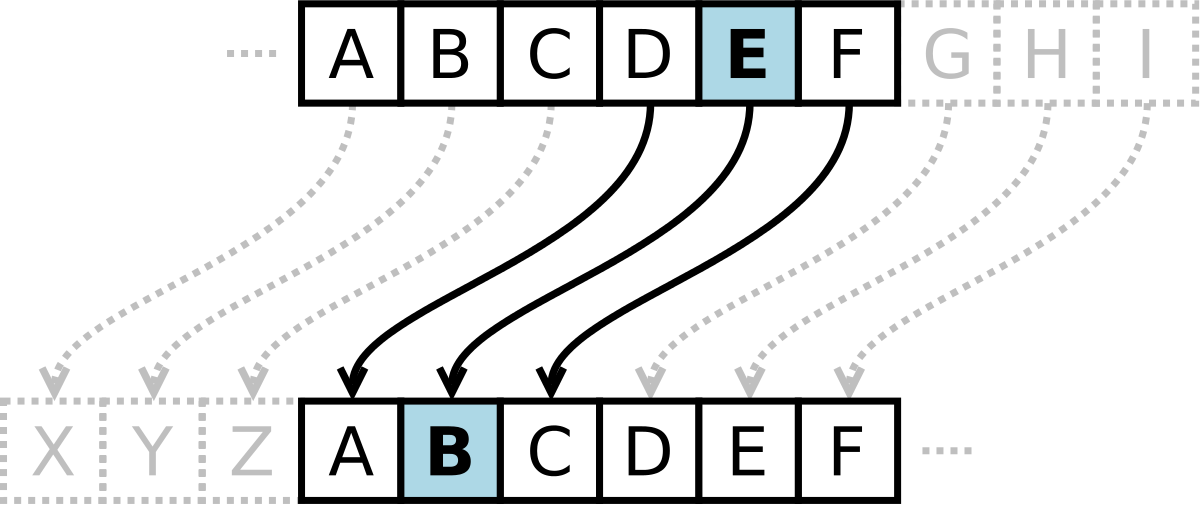
\includegraphics[width=2in]{caesar_shift.png}}
  \hspace*{.2in}
  \raisebox{-0.5\height}{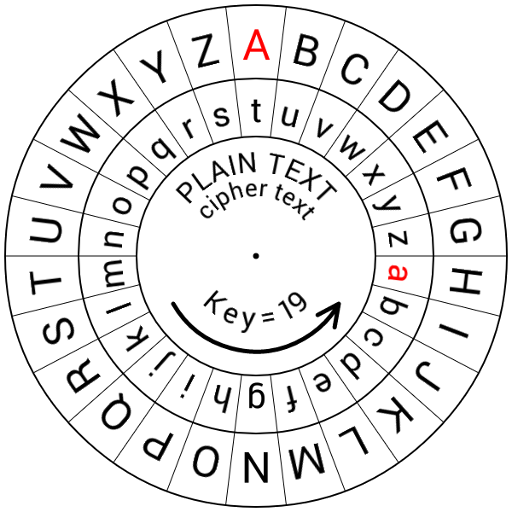
\includegraphics[width=1.5in]{caesar_wheel.png}}
\end{minipage}
\end{center}
\end{frame}

\begin{frame}
\frametitle{Mathematical notation}

First, we consider each character as an integer: $A..Z$ maps to $0..25$.

For now, just consider the plaintext as having all uppercase characters.

We denote the encryption function of some Caesar cipher of key (shift) $s$ as:
$E_s(x) = x + s \pmod{26}$

Here $a \pmod{b}$ denotes the remainder when $a$ is divided by $b$. This makes
it ``wrap around'' the way we want.
\end{frame}

\begin{frame}
\frametitle{Decryption}
If $E_s(x) = x + s \pmod{26}$, the asssociated decryption function is
$D_s(x) = x - s \pmod{26}$.

The recipient of the ciphertext already knows $s$, so they simply plug it in to
find out what the plaintext was.
\end{frame}

\subsection{The affine shift cipher}

\begin{frame}
\frametitle{Affine shift}

We now let the encryption function $E_{(a, b)}(x) = ax + b \pmod{26}$. Therefore,
\begin{align*}
D_{(a, b)}(x) &= a^{-1}(x - b) \pmod{26} \\
              &= E_{(a^{-1}, -a^{-1}b)}(x)
\end{align*}
Note that an affine shift is invertible iff $a$ is coprime to $26$
($gcd(a, 26) = 1$)
(eg consider that $E_{(2, b)}(0) = E_{(2, b)}(13) = b$).

\end{frame}

\section{Polygraph substitution ciphers}

\begin{frame}
\frametitle{Polygraph substitution}
Instead of a monograph substitution, where we have
$E(x)$, we can have for example a digraph substitition.

This means that the cipher splits the text into pairs of letters (digraphs), and
we have a function on these:
$E\left(\begin{bmatrix} x \\ y \\\end{bmatrix}\right)$
\end{frame}

\subsection{Vigen\`ere cipher}

\begin{frame}
\frametitle{Vigen\`ere cipher}

These have a key which is a sequence of letters. Each letter encodes a Caesar
shift for its corresponding letter, in essence.

An $n$-length Vigen\`ere cipher with key $k_i$ is:

$  E_{\begin{bmatrix} k_1 \\ k_2 \\ \vdots \\ k_n \end{bmatrix}}
\left(\begin{bmatrix} c_1 \\ c_2 \\ \vdots \\ c_n \end{bmatrix}\right)
   =  \begin{bmatrix}c_1 + k_1 \\ c_2 + k_2 \\ \vdots \\ c_n + k_n\end{bmatrix}
   \pmod{26}$
\end{frame}

\begin{frame}
\frametitle{Cryptanalysis}

Note that this basically leaves the shape of the distribution of every $n$th
letter, every $n + 1$th letter, and so on untouched.

If we hypothesise some key length $n$, we can therefore find the average IOC of
each of these intervals. We expect to see a reasonable spike if this is correct
(this spike will also happen for multiples of the correct $n$).
\end{frame}

\begin{frame}
\frametitle{Analysis of 2017-5b}
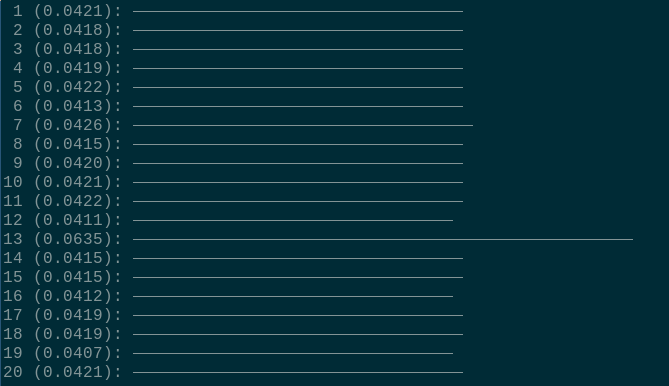
\includegraphics[width=\textwidth]{sel_screenshot_20181002_122703.png}
\end{frame}

\subsection{Other polygraph ciphers}

\begin{frame}
\frametitle{Other variants}

There are a lot of these. Really, you'll need to do some research on how to spot
each.

Some examples are:

\begin{itemize}
\item Playfair
\item Hill
\item Bifid
\end{itemize}

\end{frame}

\section{Stateful ciphers}

\begin{frame}
\frametitle{Ciphers with state}

This is most modern ciphers. These can be quite tricky. Some examples are:

\begin{itemize}
\item Autokey - this can be attacked with the techniques in this presentation.
\item Enigma (simplified). This is really mean so don't come to me for help.
\end{itemize}
\end{frame}

\end{document}
